\smalltitle{سوال 3}
\link{https://s3-us-west-2.amazonaws.com/cs188websitecontent/exams/su15\_midterm1\_solutions.pdf}{منبع}
\begin{enumerate}
    \item غلط. گراف زیر را در نظر بگیرید:
    \begin{center}
    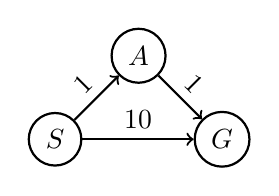
\begin{tikzpicture}[node distance={15mm}, thick, main/.style = {draw, circle}] 
        \node[main] (1) {$S$};
        \node[main] (2) [above right of=1] {$A$}; 
        \node[main] (3) [below right of=2] {$G$}; 
        \draw[->] (1) -- node[midway, above, sloped] {$1$} (2); 
        \draw[->] (2) -- node[midway, above, sloped] {$1$} (3); 
        \draw[->] (1) -- node[midway, above, sloped] {$10$} (3); 
    \end{tikzpicture} 
    \end{center}
    در این گراف ممکن است که \lr{DFS} درجا به $G$ برود و الگوریتم تمام شود با اینکه بهینه نیست.
    اما $A^*$ همیشه مسیر $SAG$ را انتخاب می‌کند.
    \item کمتر یا مساوی! در صورتی که $h = 0$ قرار دهیم الگوریتم $A^*$ مانند \lr{UCS} عمل می‌کند.
    \item غلط است. ممکن است که دو برابر کردن تابع $h$ کاری کنیم که در یکی از حالات این تابع بدبینانه بشود.
    \item بله. دقت کنید که در صورتی که $h$ \lr{admissible} باشد باید حداکثر به اندازه‌ی جواب بهینه خروجی دهد. پس $h_2$ دو برابر جواب بهینه ممکن است که خروجی دهد.
    \item درست است. چرا که با میانگین گیری صرفا $h$ هر کدام از حالات را کم می‌کنیم. پس همچنان
    \lr{admissible}
    می‌ماند.
\end{enumerate}